% Created 2024-04-25 Thu 23:58
% Intended LaTeX compiler: pdflatex
\documentclass[letterpaper]{article}
\usepackage[utf8]{inputenc}
\usepackage[T1]{fontenc}
\usepackage{graphicx}
\usepackage{longtable}
\usepackage{wrapfig}
\usepackage{rotating}
\usepackage[normalem]{ulem}
\usepackage{amsmath}
\usepackage{amssymb}
\usepackage{capt-of}
\usepackage{hyperref}
\usepackage{lmodern}
\fontsize{3pt}{4pt}\selectfont
\usepackage{amsmath}
\usepackage{amsthm}
\usepackage[left=0.5in, right=0.5in, top=0.5in, bottom=0.75in]{geometry}
\usepackage{sectsty}
\usepackage[labelformat=empty]{caption}
\usepackage{parskip}
\usepackage{mdframed}
\usepackage{caption}
\sectionfont{\centering}
\usepackage{titlesec}
\usepackage{venndiagram}
\usepackage{xcolor}
\usepackage{tikz}
\usepackage{multirow}
\usepackage{listings}
\usepackage{subcaption}
\usepackage{wrapfig}
\usepackage{graphicx}
\titleformat{\section}{\centering\large\bfseries}{\thesection}{1em}{}
\titleformat{\subsection}{\centering\large\bfseries}{\thesubsection}{1em}{}
\titleformat{\subsubsection}{\normalsize\bfseries}{1pt}{1pt}{}
\theoremstyle{definition}
\newtheorem*{theorem}{Theorem}
\newtheorem*{definition}{Definition}
\newtheorem*{lemma}{Lemma}
\newtheorem*{example}{Example}
\newtheorem*{corollary}{Corollary}
\newtheorem*{remark}{Remark}
\newtheorem*{note}{Note}
\renewcommand\qedsymbol{QED}
\usepackage{hyperref}
\hypersetup{colorlinks=true, linkcolor=magenta, urlcolor=magenta}
\usepackage{listings}
\lstset{basicstyle=\ttfamily,mathescape}
\author{Hecate}
\date{\today}
\title{}
\hypersetup{
 pdfauthor={Hecate},
 pdftitle={},
 pdfkeywords={},
 pdfsubject={},
 pdfcreator={Emacs 29.3 (Org mode 9.6.15)}, 
 pdflang={English}}
\begin{document}

\begin{center}
    \large\textsc{University of California, Los Angeles} \\
    \large\textbf{Cyrus Asasi} \\
    \large\textsc{506014946}
        
    \begin{minipage}[t]{0.5\textwidth}
        \raggedright
        \textbf{ECE M146}
    \end{minipage}%
    \begin{minipage}[t]{0.5\textwidth}
        \raggedleft
        \textbf{Prof. Suhas Diggavi}
    \end{minipage}
    \centering
    \large\textbf{Homework 6} \\
    \large\textit{Due Wednesday, April 24th, 2024 11:59pm} \textbf{via Gradescope}
\end{center}
\vspace{0.5cm}

\begin{enumerate}
\item Suppose we have a training set with 8 samples, each sample has feature vector in
\(\mathbb{R}^{2}\):
\begin{center}
\begin{tabular}{|c|c|c|c|c|c|c|c|c|}
\hline
\# & 1 & 2 & 3 & 4 & 5 & 6 & 7 & 8\\[0pt]
\hline
X & [4,0] & [1,1] & [0,1] & [-2,-2] & [-2,1] & [1,0] & [5,2] & [3,0]\\[0pt]
\hline
y & 1 & -1 & -1 & 1 & -1 & 1 & -1 & -1\\[0pt]
\hline
\end{tabular}
\end{center}

We are going to implement the perceptron algorithm to train a linear classifier with 2
dimensional weight vector \(\mathbf{w} \in \mathbb{R}^{2}\) (no bias term). We start with
initial weight vector as the first sample in our dataset, i.e. \(\mathbf{w}_{1}=\mathbf{x}_{1}\).
Note that: when \(\mathbf{w}^{\top} x=0\), the algorithm predicts +1.

To simplify the calculation, you only need to test and possibly update each sample once in the
given sequence. You can either implement the algorithm by hand or programming.

\begin{enumerate}
\item Is the data linearly separable?
Will our algorithm converge if we run it several times over the same sequence? Explain.

\color{teal}
By observing figure 1, we can clearly see that the dataset is not linearly separable.
Since the dataset is not linearly separable, the perceptron learning algorithm will not
converge. This can be illustrated by figure 2, which was generated by running the perceptron
algorithm 100 times on the data set and assigning a newly colored line corresponding to each
updated vector \(\mathbf{w}\).
\color{black}

\begin{figure}[htbp]
\centering
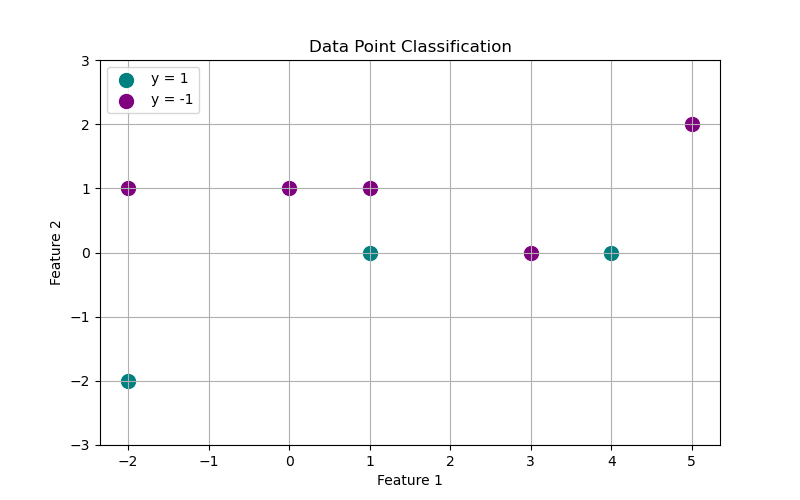
\includegraphics[width=250]{../assets/hw1_fig1.png}
\caption{Figure 1: Plot of dataset.}
\end{figure}

\begin{figure}[htbp]
\centering
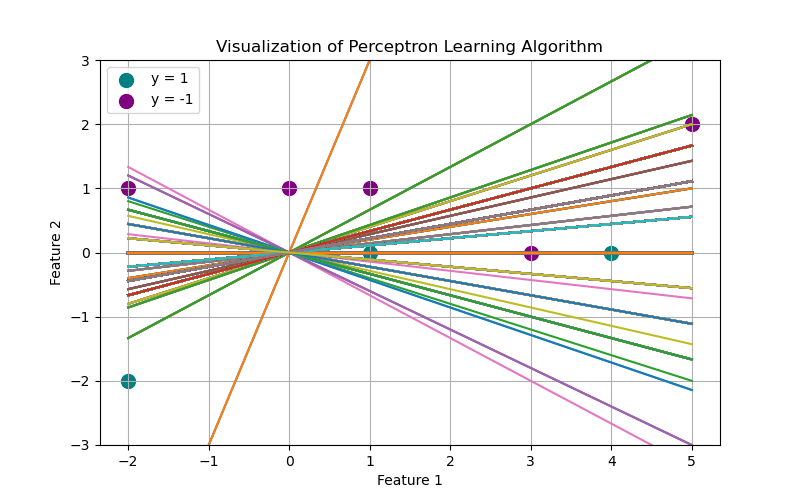
\includegraphics[width=250]{../assets/hw1_fig2.png}
\caption{Figure 2: Plot of perception learning algorithm run 100 times.}
\end{figure}

\item Regardless of whether the dataset is linearly separable or not, calculate the updates of the
weight vector on this sequence for one round over the entire dataset.
Follow the order of the index for the samples and show your calculations.

\color{teal}
\begin{align*}
w_0 &= [4, 0] \quad \text{initial} \\
w_1 &= [4, 0] \quad \text{no update} \\
w_2 &= [4, 0] + -1 * [1, 1] = [3, -1] \quad \text{update} \\
w_3 &= [3, -1] \quad \text{no update} \\
w_4 &= [3, -1] + 1 * [-2, -2] = [1, -3] \quad \text{update} \\
w_5 &= [1, -3] \quad \text{no update} \\
w_6 &= [1, -3] \quad \text{no update} \\
w_7 &= [1, -3] \quad \text{no update} \\
w_8 &= [1, -3] + -1 * [3, 0] = [-2, -3] \quad \text{update} 
\end{align*}
\color{black}

\item Provide closed-form functions for the perceptron, Voted perceptron,
and Average perceptron, using the weight vector(s) derived in part (b).
\color{teal}
\begin{enumerate}
\item Perceptron:
The perceptron algorithm updates the weight vector when a mistake is made.
We can use the final weight vector to construct a closed-form function for
future predictions.
$$f(\mathbf{x}) = sign(\mathbf{w}^T\mathbf{x}) = sign([-2, -3] \cdot \mathbf{x})$$
\item Voted Perceptron:
The voted perceptron maintains a list of weight vectors along with the number of times
each one 'voted' for a correct classification before an update was needed.

\begin{align*}
f(\mathbf{x}) &= sign\left[\sum_{i=1} s_i \cdot sign(\mathbf{w}_i^T \mathbf{x})\right] \\
&= sign \left[2 \cdot sign([4, 0] \cdot \mathbf{x}) + 2 \cdot sign([3, -1] \cdot \mathbf{x}) +
4 \cdot sign( [1, -3]\cdot \mathbf{x}) + 1 \cdot sign([-2, -3]) \cdot \mathbf{x} \right]
\end{align*}

\item Average Perceptron:
The average perceptron takes the average of all the weight vectors across updates.
This weighted average vector is:

\begin{align*}
f(\mathbf{x}) &= sign \left[ \sum_{i=1} s_i \cdot \mathbf{w}_i^T \mathbf{x}\right] \\
&= sign \left[2 \cdot [4, 0] \cdot \mathbf{x} + 2 \cdot [3, -1] \cdot \mathbf{x} +
4 \cdot [1, -3] \cdot \mathbf{x} + 1 \cdot [-2, -3] \cdot \mathbf{x} \right]
\end{align*}
\end{enumerate}

\color{black}

\item Using the functions derived in part (c), compare the errors between the perceptron,
the Voted perceptron predictor, and the Average perceptron predictor across the entire dataset.
For each point in the dataset, find the label assigned by each classifier and report the error
over the dataset.

\color{teal}
\begin{table}[htbp]
\caption{\(y_i\) is perceptron, \(y_{ii}\) is voted, \(y_{iii}\) is averaged}
\centering
\begin{tabular}{|c|c|c|c|c|c|c|c|c|}
\hline
\hline
\# & 1 & 2 & 3 & 4 & 5 & 6 & 7 & 8\\[0pt]
\hline
X & [4,0] & [1,1] & [0,1] & [-2,-2] & [-2,1] & [1,0] & [5,2] & [3,0]\\[0pt]
\hline
y & 1 & -1 & -1 & 1 & -1 & 1 & -1 & -1\\[0pt]
\hline
\(y_i\) & -1 & -1 & -1 & 1 & 1 & -1 & -1 & -1\\[0pt]
\hline
\(y_{ii}\) & 1 & -1 & -1 & 1 & -1 & 1 & -1 & 1\\[0pt]
\hline
\(y_{iii}\) & 1 & -1 & -1 & 1 & -1 & 1 & 1 & 1\\[0pt]
\hline
\hline
\end{tabular}
\end{table}

\begin{verbatim}
Perceptron Error Rate: 0.375
Voted Perceptron Error Rate: 0.125
Average Perceptron Error Rate: 0.25
\end{verbatim}
\color{black}
\end{enumerate}

\item In class, we have seen the logistic regression when labels are \(\{0,1\}\). In this question,
you will derive the logistic regression when labels are instead \(\{-1,1\}\).

In class, we considered the dataset \(\mathcal{D}=\left\{\left(\mathbf{x}_{1}, y_{1}\right), \ldots,\left(\mathbf{x}_{n}, y_{n}\right)\right\}\) with \(n\) samples where \(\mathbf{x}_{i} \in \mathbb{R}^{d}\) and labels \(y_{i} \in\{0,1\}\) for all \(i \in[n]\). The prediction function \(h_{\mathbf{w}}(\mathbf{x})\) studied in class is given by

\begin{equation*}
h_{\mathbf{w}}(\mathbf{x})=\frac{1}{1+e^{-\mathbf{w}^{\top} \mathbf{x}}}=\frac{e^{\mathbf{w}^{\top} \mathbf{x}}}{1+e^{\mathbf{w}^{\top} \mathbf{x}}} \tag{1}
\end{equation*}

Moreover, the objective studied in class to minimize for logistic regression was:

\begin{equation*}
\text { P2.1: } \quad \min _{\mathbf{w}}-\sum_{i=1}^{n}\left[y_{i} \log \left(h_{\mathbf{w}}\left(\mathbf{x}_{i}\right)\right)+\left(1-y_{i}\right) \log \left(1-h_{\mathbf{w}}\left(\mathbf{x}_{i}\right)\right)\right] \tag{2}
\end{equation*}

We want to modify this objective function so that \(\tanh _{\mathbf{w}}(\mathbf{x})=\frac{e^{\mathbf{w}^{\top} \mathbf{x}}-e^{-\mathbf{w}^{\top} \mathbf{x}}}{e^{\mathbf{w}^{\top} \mathbf{x}}+e^{-\mathbf{w}^{\top} \mathbf{x}}}=\frac{e^{2 \mathbf{w}^{\top} \mathbf{x}}-1}{e^{2 \mathbf{w}^{\top} \mathbf{x}}+1}\) is the activation function and \(\tilde{y}_{i} \in\{-1,1\}\) the labels.

\begin{enumerate}
\item Show that

$$
      \tanh _{\mathbf{w}}(\mathbf{x})=2 h_{\mathbf{w}^{\prime}}(\mathbf{x})-1, \mathbf{w}^{\prime}=2 \mathbf{w}
      $$

\color{teal}
$$
      h_{\mathbf{w}'}(\mathbf{x}) = h_{2\mathbf{w}}(x) = \frac{e^{2\mathbf{w}^T\mathbf{x}}}{1 + e^{2\mathbf{w}^T\mathbf{x}}}
      $$

$$
      2h_{\mathbf{w}'}(\mathbf{x}) - 1 = \frac{2e^{2\mathbf{w}^T\mathbf{x}}}{1 + e^{2\mathbf{w}^T\mathbf{x}}} -
      \frac{1 + e^{2\mathbf{w}^T\mathbf{x}}}{1 + e^{2\mathbf{w}^T\mathbf{x}}}
      = \frac{e^{2 \mathbf{w}^{\top} \mathbf{x}}-1}{e^{2 \mathbf{w}^{\top} \mathbf{x}}+1}
      $$
Therefore, \(\tanh _{\mathbf{w}}(\mathbf{x})=2 h_{\mathbf{w}^{\prime}}(\mathbf{x})-1\)

\color{black}

\item What are the asymptotic values of the function \(\tanh _{\mathbf{w}}(\mathbf{x})\) as \(\mathbf{w}^{\top} \mathbf{x} \rightarrow \infty\) and \(\mathbf{w}^{\top} \mathbf{x} \rightarrow-\infty\)? Roughly draw the graph of this function with respect to \(\mathbf{w}^{\top} \mathbf{x}\). What is the decision criterion you can choose for predicting labels as -1 or 1?

\color{teal}
The asymptotic values of the \(tanh_{\mathbf{w}}(\mathbf{x})\) as
\(\mathbf{w}^{\top} \mathbf{x} \rightarrow \infty\) and
\(\mathbf{w}^{\top} \mathbf{x} \rightarrow-\infty\) are 1 and -1 respectively.

\begin{figure}[htbp]
\centering
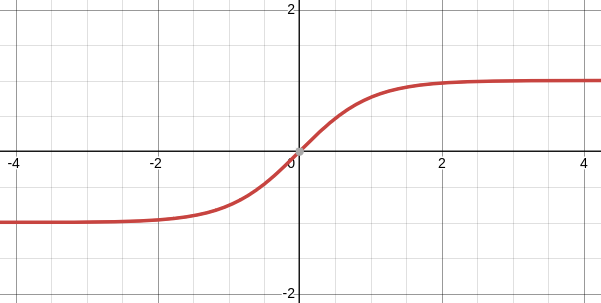
\includegraphics[width=400]{../assets/hw1_fig3.png}
\caption{Figure 3: Graph of \(tanh_{\mathbf{w}}(\mathbf{x})\)}
\end{figure}

A good decision criteria for predicting lables as -1 or 1 can be defined as follows.
$$\text{label classifier} = \begin{cases}1 & x \ge 0 \\ -1 & x < 0 \end{cases}$$

\color{black}

\item Using your answer in part (b), argue that we cannot directly replace \(h_{\mathbf{w}}\left(\mathbf{x}_{i}\right)\) with \(\tanh _{\mathbf{w}}(\mathbf{x})\) in the optimization problem P2.1.

\color{teal}
We cannot use \(tanh_{\mathbf{w}}(\mathbf{x})\) to replace
\(h_{\mathbf{w}}\left(\mathbf{x}_{i}\right)\) because logarithms of negative numbers are not
defined. While \(h_{\mathbf{w}}\left(\mathbf{x}_{i}\right)\) remains positive,
\(tanh_{\mathbf{w}}(\mathbf{x})\) drops below zero when \(x < 0\). This makes it impossible
to use \(tanh_{\mathbf{w}}(\mathbf{x})\) in the optimization problem P2.1.
\color{black}

\item When labels are \(\tilde{y}_{i} \in\{-1,1\}\) show, using your answer in part (a), that the optimization problem in P2.1 is equivalent to:

\begin{equation*}
\text { P2.2: } \quad \min _{\mathbf{w}}-\sum_{i=1}^{n}\left[\frac{1+\tilde{y}_{i}}{2} \log \left(\frac{1+\tanh _{\mathbf{w}}\left(\mathbf{x}_{i}\right)}{2}\right)+\frac{1-\tilde{y}_{i}}{2} \log \left(\frac{1-\tanh _{\mathbf{w}}\left(\mathbf{x}_{i}\right)}{2}\right)\right] \tag{3}
\end{equation*}

\color{teal}
\(\frac{1 + \tilde{y}_{i}}{2}\) and \(\frac{1 - \tilde{y}_{i}}{2}\) essentially modify P2.2 so
that it has the same behavior as the \(y_i\) and \((1-y_i)\) in P2.1, except that it works when
the values of \(y\) are 1 and -1, rather than 1 and 0.

To show that P2.2 for \(\tilde{y}_i \in \{-1, 1\}\) is the same as P2.1, we also need to show
that the following two identities hold. However, both of these have already been proven in
part a). By substituting \(\tanh _{\mathbf{w}}(\mathbf{x})=2 h_{\mathbf{w}^{\prime}}(\mathbf{x})-1\),
we can clearly see that both identities hold.

\begin{align*}
&\log \left[\frac{1+\tanh _{\mathbf{w}}\left(\mathbf{x}_{i}\right)}{2}\right] =
\log \left(h_{\mathbf{w}}\left(\mathbf{x}_{i}\right)\right) \\
&\log \left[\frac{1-\tanh _{\mathbf{w}}\left(\mathbf{x}_{i}\right)}{2}\right] =
\log \left(1 - h_{\mathbf{w}}\left(\mathbf{x}_{i}\right)\right) \\
\end{align*}
\color{black}

\item Compute the gradient of the loss function in P2.2 (3) for a single sample \(\mathbf{x}_{i}\). Consider the two cases \(\tilde{y}_{i}=1\) and \(\tilde{y}_{i}=-1\) separately.

\color{teal}

For \(\tilde{y}_i = 1\):

$$
      L(\mathbf{w}) = -\left[ \log \left(\frac{1+\tanh(\mathbf{w}^\top \mathbf{x}_i)}{2}\right)\right]
      $$

\begin{align*}
\frac{\partial L}{\partial \mathbf{w}} & = -\left( \frac{2}{1 + \tanh(\mathbf{w}^\top \mathbf{x}_i)} \right) \left(\frac{1 - \tanh^2(\mathbf{w}^\top \mathbf{x}_i)}{2}\right) \frac{\partial}{\partial \mathbf{w}} (\mathbf{w}^\top \mathbf{x}_i) \\
& = -\left( \frac{1 - \tanh^2(\mathbf{w}^\top \mathbf{x}_i)}{1 + \tanh(\mathbf{w}^\top \mathbf{x}_i)} \right) \mathbf{x}_i
\end{align*}

For \(\tilde{y}_i = -1\):

$$
      L(\mathbf{w}) = -\left[ \log \left(\frac{1-\tanh(\mathbf{w}^\top \mathbf{x}_i)}{2}\right)\right]
      $$

\begin{align*}
\frac{\partial L}{\partial \mathbf{w}} & = -\left( \frac{2}{1 - \tanh(\mathbf{w}^\top \mathbf{x}_i)} \right) \left(\frac{1 - \tanh^2(\mathbf{w}^\top \mathbf{x}_i)}{2}\right) \frac{\partial}{\partial \mathbf{w}} (\mathbf{w}^\top \mathbf{x}_i) \\
& = -\left( \frac{1 - \tanh^2(\mathbf{w}^\top \mathbf{x}_i)}{1 - \tanh(\mathbf{w}^\top \mathbf{x}_i)} \right) \mathbf{x}_i
\end{align*}
\end{enumerate}

\item In each of these problems, give a clear explanation for your choice.

\begin{enumerate}
\item \textbf{Perceptrons}:

\begin{enumerate}
\item When the perceptron algorithm encounters an incorrectly classified sample \(\left(\mathbf{x}_{i}, y_{i}\right)\) with weights \(\mathbf{w}\), it updates the weights and obtains \(\mathbf{w}^{\prime}\) after the update. \(\mathbf{w}^{\prime}\) correctly classifies \(\left(\mathbf{x}_{i}, y_{i}\right)\).

\color{teal}
\textbf{FALSE}. The perceptron algorithm does not guarantee that \(\mathbf{w}'\) will be correct
after the update. It only guarantees that \(\mathbf{w}'\) will be closer to correctly
classifying a sample.
\color{black}
\item If the data is linearly seperable, then the Rosenblatt perceptron algorithm converges to a solution that makes no errors on the training data.

\color{teal}
\textbf{TRUE}. The perceptron algorithm will eventually converge to a solution that correctly
classifies all points in a linearly seperable dataset because it iteratively adjusts
the weights and bias to correctly classify all data points.
\color{black}

\item For a perceptron classifier with weights \(\mathbf{w}\), the prediction made on a feature
\(\mathbf{x}\) is \(sign\left(\mathbf{w}^{\top}\mathbf{x}\right)\).
If we multiply the weights obtained from perceptron by a negative scalar,
this flips all predictions made by the perceptron algorithm.

\color{teal}
\textbf{FALSE}. Simply multiplying the weights by a negative scalar will not flip all
predictions made by the perceptron algorithm because if \(\mathbf{w}^T\mathbf{x}\)
happens to be 0, multiplying it by a negative scalar will not change the prediction.
\color{black}
\end{enumerate}

\item \textbf{Logistic Regression}:

\begin{enumerate}
\item The prediction of a logistic regression classifier is given by
\(y=\sigma\left(\mathbf{w}^{\top} \mathbf{x}\right) \in[0,1]\).
Moreover, the decision boundary of this classifier is
\(\mathbf{w}^{\top} \mathbf{x} \geq 0\).

\color{teal}
\textbf{TRUE}. The decision boundary is when \(\sigma\mathbf{w}^T{\mathbf{x} = 0.5\) which
corresponsds to when \(\mathbf{w}^T\mathbf{x} = 0\). The sigmoid function works as
defined by the problem, and is defined on [0, 1].
\color{black}

\item The stochastic gradient descent optimization is more computationally efficient than
batch gradient descent per iteration.

\color{teal}
\textbf{TRUE}. This is definitely the case because stochastic gradient descent chooses a single
random point rather than considering all points when calculating loss and derivative.
\color{black}

\item Let \(h_{\mathbf{w}}(\mathbf{x})=\mathbf{w}^{\top} \mathbf{x},(\mathbf{x}, y)\) a sample,
and \(\sigma(a)=\frac{1}{1+e^{-a}}\). When \(y=0\), it is true that

$$
	 -y \log \left(\sigma\left(h_{\mathbf{w}}(\mathbf{x})\right)\right)-(1-y) \log \left(1-\sigma\left(h_{\mathbf{w}}(\mathbf{x})\right)\right)=\log \left(1+e^{h_{\mathbf{w}}(\mathbf{x})}\right)-1_{y=1} h_{\mathbf{w}}(\mathbf{x})
	 $$

\color{teal}
\textbf{TRUE}.
When \(y = 0\)
\begin{align*}
-y \log \left(\sigma\left(h_{\mathbf{w}}(\mathbf{x})\right)\right)-(1-y) \log \left(1-\sigma\left(h_{\mathbf{w}}(\mathbf{x})\right)\right)
&= -\log \left(1-\sigma\left(h_{\mathbf{w}}(\mathbf{x})\right)\right) \\
&= -\log\left(1 - \frac{1}{1 + e^{-h_{\mathbf{w}}(\mathbf{x})}}\right) \\
&= -\log\left(\frac{e^{-h_{\mathbf{w}}(\mathbf{x})}}{1 + e^{-h_{\mathbf{w}}(\mathbf{x})}}\right) \\
&= -\left[\log(e^{-h_{\mathbf{w}}(\mathbf{x})}) - \log(1 + e^{-h_{\mathbf{w}}(\mathbf{x})})\right] \\
&= h_{\mathbf{w}}(\mathbf{x}) + \log(1 + e^{-h_{\mathbf{w}}(\mathbf{x})}) \\
&= \log(1 + e^{h_{\mathbf{w}}(\mathbf{x})}) \\
&= \log(1 + e^{h_{\mathbf{w}}(\mathbf{x})}) - 1_{y=1} h_{\mathbf{w}}(\mathbf{x})
\end{align*}
\(1_{y=1} = 0\) when \(y = 0\)
\color{black}

\item Let \(\sigma(a)=\frac{1}{1+e^{-a}}\), then the derivative is
\(\frac{d \sigma(a)}{d a}=\frac{-1+e^{-a}}{\left(1+e^{-a}\right)^{2}}\).

\color{teal}
\textbf{FALSE}. The derivative of the sigmoid function \(\sigma(a)\) is
$$
	 \sigma(a) \cdot (1 - \sigma(a)) \implies \frac{1}{1 + e^{-a}} \cdot \left(1 - \frac{1}{1 + e^{-a}}\right)
	 = \frac{e^{-a}}{(1 + e^{-a})^2} \ne \frac{-1 + e^{-a}}{(1 + e^{-a})^2}
	 $$
\color{black}
\end{enumerate}

\item \textbf{Linear Regression}:

\begin{enumerate}
\item A closed form solution for linear regression is only possible if \(\boldsymbol{X}^{\top} \boldsymbol{X}\) is positive definite. Note that a matrix \(\boldsymbol{A}\) is positive definite if \(\mathbf{z}^{\top} \boldsymbol{A} \mathbf{z}>0\) for all vectors \(\mathbf{z} \neq \mathbf{0}\)

\color{teal}
\textbf{FALSE}. A closed form solution for linear regression is possible if
\(\mathbf{X}^T\mathbf{X}\) is positive semi-definite and invertible.
\color{black}

\item The loss function of \(\ell_{2}\) regularized linear regression is \(\|\boldsymbol{X} \mathbf{w}-\mathbf{y}\|_{2}^{2}+\lambda\|\mathbf{w}\|_{2}^{2}\). The gradient of the loss function with respect to \(\mathbf{w}\) is given by \(2 \boldsymbol{X}^{\top}(\boldsymbol{X} \mathbf{w}-\mathbf{y})+2 \lambda \mathbf{w}\).

\color{teal}
\textbf{TRUE}. The derivative computation below shows the validity of the above statement.
\begin{align*}
\frac{\partial}{\partial \mathbf{w}} \|\boldsymbol{X} \mathbf{w}-\mathbf{y}\|_{2}^{2}+ \frac{\partial}{\partial \mathbf{w}} \lambda\|\mathbf{w}\|_{2}^{2}
&= \frac{\partial}{\partial \mathbf{w}} \left[(\boldsymbol{X}\mathbf{w} - \mathbf{y})^{\top}(\boldsymbol{X}\mathbf{w} - \mathbf{y})\right] +
\frac{\partial}{\partial \mathbf{w}} \lambda (\mathbf{w}^T\mathbf{w}) \\
&= \frac{\partial}{\partial \mathbf{w}} \left[(\mathbf{X}^T\mathbf{w}^T - \mathbf{y}^T)(\mathbf{Xw} - \mathbf{y})\right]  + 2\lambda\mathbf{w} \\
&= \frac{\partial}{\partial \mathbf{w}} \left[\mathbf{w}^\top \boldsymbol{X}^\top \boldsymbol{X} \mathbf{w} - \mathbf{w}^\top \boldsymbol{X}^\top \mathbf{y} - \mathbf{y}^\top \boldsymbol{X} \mathbf{w} + \mathbf{y}^\top \mathbf{y}\right] + 2\lambda\mathbf{w}\\
&= 2\mathbf{X}^T\mathbf{Xw} - 2\mathbf{X}^T\mathbf{y} + 0 + 2\lambda\mathbf{w} \\
&= 2\mathbf{X}^T(\mathbf{Xw} - \mathbf{y}) + 2\lambda\mathbf{w}
\end{align*}

\color{black}
\end{enumerate}
\end{enumerate}

\item In this exercise, you will work through a family of binary classifications.
Our data consists of inputs \(x_{n} \in \mathbb{R}^{1 \times d}\) and labels \(y_{n} \in\{-1,1\}\)
for \(n \in\{1, \ldots, N\}\). We will work on a subset of the Fashion-MNIST dataset which focuses
on classifying whether the image is for a Dress \((y=1)\) or a Shirt \((y=-1)\).Your goal is to
learn a classifier based on linear predictor \(h_{\mathbf{w}}(x)=\mathbf{w}^{T} x\). Let
\begin{equation}
\mathbf{X}=\left[\begin{array}{c}
x_{1}  \tag{4}\\
\vdots \\
x_{N}
\end{array}\right] \in \mathbb{R}^{N \times d}, \quad \mathbf{y}=\left[\begin{array}{c}
y_{1} \\
\vdots \\
y_{N}
\end{array}\right] \in\{1,-1\}^{N}
\end{equation}
The main file is the Notebook Jupyter notebook.

\begin{enumerate}
\item (\textbf{Visualization}): Visualize a sample of the training data. What is the dimensions of \(X_{\text {train }}\), and \(X_{\text {test }}\).

\color{teal}
The dimensions of \(X_{\text{train}} = (5000, 784)\) and the dimensions of \(X_{\text{test}} = (500, 784)\).
\color{black}

\item (\textbf{Perceptron}): Implement Perceptron Algorithm to classify your training data.
Let the maximum number of iterations of the Algorithm num \(_{\text {iter }}=N\) (number of training samples).
At each iteration, compute the percentage of misclassified points in the training dataset,
and save it into a \texttt{Loss\_hist} array. Plot the history of the loss function (\texttt{Loss\_hist}).
What is the final value of the loss function and the squared \(\ell_{2}\) norm value of the weight \(\|\mathbf{w}\|_{2}^{2}\) ? Looking at the loss function, can you comment on whether the Perceptron algorithm converges?

\color{teal}
\begin{figure}[htbp]
\centering
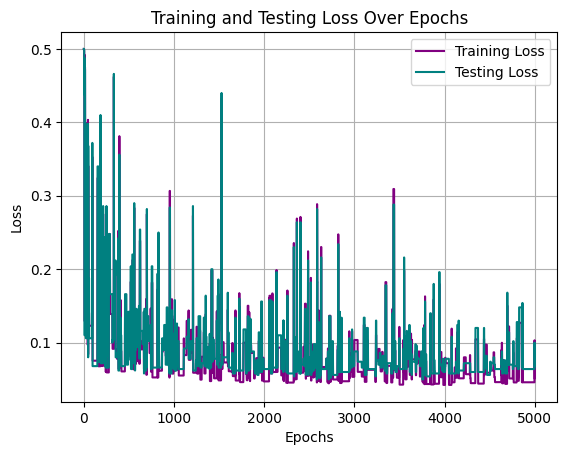
\includegraphics[width=400]{../assets/hw1_fig4.png}
\caption{Figure 4: Perceptron Training Loss Over Iterations}
\end{figure}
The final value of the loss function was \(5.16\%\) missclassified, while the final \(\ell 2\) norm
value of the weight vector was \(1404179381\). From Figure 4 and the loss function, we can
clearly see that the perceptron algorithm does not converge.
\color{black}

\item (\textbf{Perceptron test error}): Compute the percentage of misclassified points in the test data
for the trained Perceptron.
\color{teal}
The percentage of misclassified points in the test data after training the perceptron is
\(6.80\%\).
\color{black}

\item (\textbf{Logistic Regression}): In this part, we will implement the logistic regression for binary
classification. Recall that logistic regression attempts to minimize the objective function
\begin{equation*}
J(\mathbf{w})=\frac{1}{N}
\left(\sum_{n=1}^{N} \log \left(1+e^{h_{\mathbf{w}}\left(\mathbf{x}_{n}\right)}\right)-
\sum_{n=1}^{N} \mathbf{1}_{y_{n}=1} h_{\mathbf{w}}\left(\mathbf{x}_{n}\right)\right) \tag{5}
\end{equation*}

where \(\mathbf{x}_{n}=\left(1, x_{n}\right)\), and \(\mathbf{1}_{A}=1\) if \(A\) is true and 0
otherwise. Moreover,
\(h_{\mathbf{w}}\left(\mathbf{x}_{n}\right)=\mathbf{w}^{T} \mathbf{x}_{n}\).
First, we will add an additional feature to each instance and set it to one.
This is equivalent to adding an additional first column to \(\mathbf{X}\) and
setting it to all ones. Modify the \texttt{get\_features()} in
\texttt{Logistic.py} file to create a matrix \(\mathbf{X}\) for logistic regression model.

\item Complete predict() in \texttt{Logistic.py} file to predict \(\mathbf{y}\) from \(\mathbf{X}\) and
\(\mathbf{w}\).

\item Complete the function \texttt{loss\_and\_grad()} to compute the loss function and the gradient of the
loss function with respect to \(\mathbf{w}\) for a data set \(\mathbf{X}\) and labels
\(\mathbf{y}\) at given weights \(\mathbf{w}\). Test your results by running the code in the
main file \texttt{Notebook.ipynb}. If you implement everything correctly, you should get the loss
function within 0.7 and squared \(\ell_{2}\) norm of the gradient around \(1.8 \times 10^{5}\).

\item Complete the function \texttt{train\_LR()} to train the logistic regression model for given learning
rate \(\eta=10^{-6}\), \texttt{batch\_size} \(=100\), and number of iterations num
\(_{\text {iters }}=5000\). Plot the history of the loss function (\texttt{Loss\_hist}).
What is the final value of the loss function and the squared \(\ell_{2}\) norm value of the
weight \(\|\mathbf{w}\|_{2}^{2}\)?

\color{teal}
\begin{figure}[htbp]
\centering
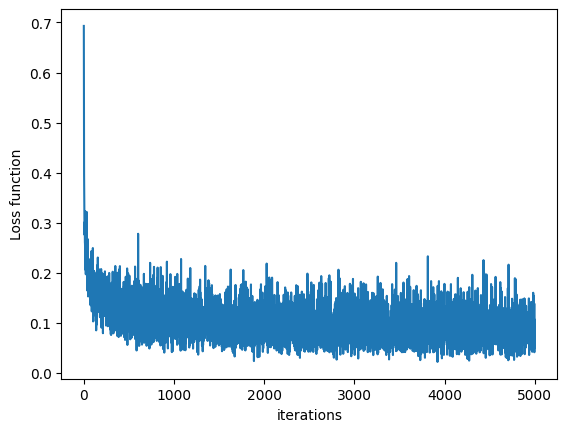
\includegraphics[width=400]{../assets/hw1_fig5.png}
\caption{Figure 5: History of the Loss Function}
\end{figure}

The final value of the loss function is \(0.0694\) \\[0pt]
The squared \(\ell_2\) norm value of the weight is \(0.000287\)
\color{black}

\item (\textbf{Logistic Regression test error}): Compute the percentage of misclassified points in the
test data for the trained Logistic Regression.

\color{teal}
The percentage of misclassified points in the test data calculated by the predict function
is \(6.6\%\)
\color{black}

\item (\textbf{Logistic Regression and Batch Size}): Train the Logistic regression model with different
batch size \(b \in\{1,50,100,200,300\}\), learning rate \(\eta=10^{-5}\), and number of
iterations \(num_{iter} = 6000/b\). Train each model 50 or 100 times and average the test error
for each value of batch size. Plot the test error as a function of the batch size.
Which batch size gives the minimum test error?

\color{teal}
\begin{figure}[htbp]
\centering
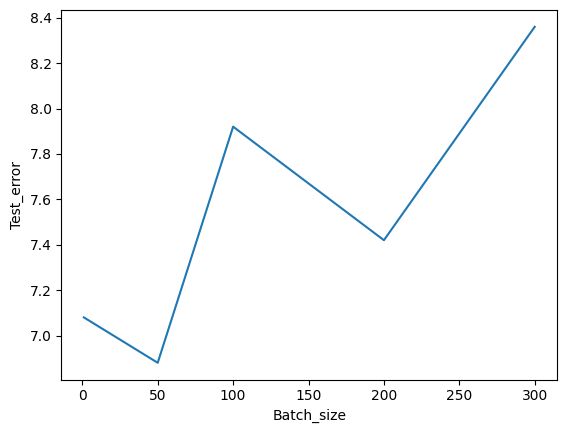
\includegraphics[width=400]{../assets/hw1_fig6.png}
\caption{Figure 6: Test Error for Batch Logistic Regression}
\end{figure}

From the graph of the error, we can clearly see that the batch size of 50 gives the minimum
error.
\color{black}
\end{enumerate}

\item In this exercise, you will work through linear and polynomial regression. Our data consists of inputs \(x_{n} \in \mathbb{R}\) and outputs \(y_{n} \in \mathbb{R}, n \in\{1, \ldots, N\}\), which are related through a target function \(y=f(x)\). Your goal is to learn a linear predictor \(h_{\mathbf{w}}(x)\) that best approximates \(f(x)\). \\[0pt]

\textbf{Visualization} \\[0pt]

As we learned last week, it is often useful to understand the data through visualizations. For this data set, you can use a scatter plot to visualize the data since it has only two properties to plot ( \(x\) and \(y\) ). \\[0pt]

\textbf{Linear Regression} \\[0pt]

Recall that linear regression attempts to minimize the objective function

$$
   J(\mathbf{w})=\sum_{n=1}^{N}\left(h_{\mathbf{w}}\left(\mathbf{x}_{n}\right)-y_{n}\right)^{2}
   $$

In this problem, we will use the matrix-vector form where

$$
   \mathbf{y}=\left(\begin{array}{c}
   y_{1} \\
   y_{2} \\
   \vdots \\
   y_{N}
   \end{array}\right), \quad \boldsymbol{X}=\left(\begin{array}{c}
   \mathbf{x}_{1}^{\top} \\
   \mathbf{x}_{2}^{\top} \\
   \vdots \\
   \mathbf{x}_{N}^{\top}
   \end{array}\right), \quad \mathbf{w}=\left(\begin{array}{c}
   w_{0} \\
   w_{1} \\
   w_{2} \\
   \vdots \\
   w_{D}
   \end{array}\right)
   $$

and each instance \(\mathbf{x}_{n}=\left(1, x_{n, 1}, \ldots, x_{n, D}\right)^{\top}\).

In this instance, the number of input features \(D=1\).

Rather than working with this fully generalized, multivariate case, let us start by considering a simple linear regression model:

$$h_{\mathbf{w}}(\mathbf{x})=\mathbf{w}^{\top} \mathbf{x}=w_{0}+w_{1} x_{1}$$

\texttt{regression.py} contains the skeleton code for the class Regression.
Objects of this class can be instantiated as model \(=\) Regression (m)
where \(m\) is the degree of the polynomial feature vector where the feature vector for instance
\(n,\left(1, x_{n, 1}, x_{n, 1}^{2}, \ldots, x_{n, 1}^{m}\right)^{\top}\). Setting \(m=1\)
instantiates an object where the feature vector for instance
\(n,\left(1, x_{n, 1}\right)^{\top}\).

\begin{enumerate}
\item Visualize the training and test data using the \texttt{plot\_data(...)} function.
What do you observe? For example, can you make an educated guess on the effectiveness of
linear regression in predicting the data?

\color{teal}
\begin{figure}[htbp]
\centering
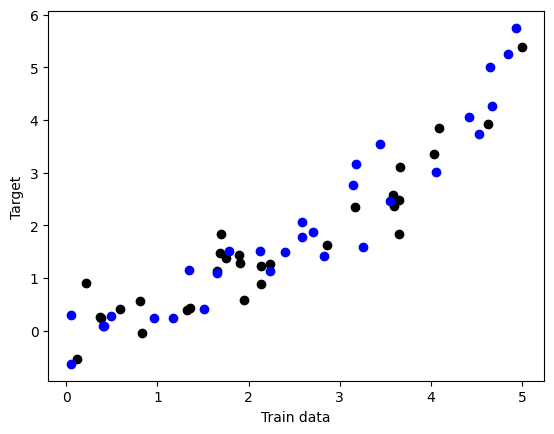
\includegraphics[width=400]{../assets/hw1_fig7.png}
\caption{Figure 7: Visualization of Data For Linear Regression}
\end{figure}

The scatter plot shows a nonlinear, possibly polynomial or exponential trend. Linear regression may not effectively predict this data due to its non-linearity; a nonlinear model would likely be more appropriate.
\color{black}

\item Note that to take into account the intercept term \(\left(w_{0}\right)\), we can add an additional "feature" to each instance and set it to one, e.g. \(x_{i, 0}=1\). This is equivalent to adding an additional first column to \(\boldsymbol{X}\) and setting it to all ones.

Modify \texttt{get\_poly\_features()} in \texttt{Regression.py} for the case \(m=1\) to create the matrix
\(\boldsymbol{X}\) for a simple linear model.

\color{teal}
See code in appendix
\color{black}

\item Before tackling the harder problem of training the regression model, complete predict()
in \texttt{Regression.py} to predict \(\mathbf{y}\) from \(\boldsymbol{X}\) and \(\mathbf{w}\).

\color{teal}
See code in appendix
\color{black}

\item One way to solve linear regression is through gradient descent (GD).

Recall that the parameters of our model are the \(w_{j}\) values.
These are the values we will adjust to minimize \(J(\mathbf{w})\).
In gradient descent, each iteration performs the update

$$w_{j} \leftarrow w_{j}-2 \eta \sum_{n=1}^{N}\left(h_{\mathbf{w}}\left(\mathbf{x}_{n}\right)-y_{n}\right) x_{n, j} \quad\left(\text { simultaneously update } w_{j} \text { for all } j\right) .$$

With each step of gradient descent, we expect our updated parameters \(w_{j}\) to come closer to the parameters that will achieve the lowest value of \(J(\mathbf{w})\).

\begin{itemize}
\item As we perform gradient descent, it is helpful to monitor the convergence by computing the
loss, i.e., the value of the objective function \(J\). Complete \texttt{loss\_and\_grad()}
to calculate \(J(\mathbf{w})\), and the gradient. Test your results by running the code
in the main file Notebook.ipnyb. If you implement everything correctly,
you should get the loss function around 4 and gradient approximately \([-3.2,-10.5]\).
\end{itemize}

We will use the following specifications for the gradient descent algorithm:

\begin{itemize}
\item We run the algorithm for 10,000 iterations.
\item We will use a fixed step size.
\item So far, you have used a default learning rate (or step size) of \(\eta=0.01\).
Try different \(\eta=10^{-4}, 10^{-3}, 10^{-1}\), and make a table of the coefficients
and the final value of the objective function. How do the coefficients compare?

\color{teal}
The coefficients were all about the same in terms of loss
\color{black}
\end{itemize}

\item In class, we learned that the closed-form solution to linear regression is

$$
      \mathbf{w}=\left(\boldsymbol{X}^{\top} \boldsymbol{X}\right)^{-1} \boldsymbol{X}^{\top} \mathbf{y}
      $$

Using this formula, you will get an exact solution in one calculation: there is no
"loop until convergence" like in gradient descent.

\begin{itemize}
\item Implement the closed-form solution \texttt{closed\_form()}.
\item What is the closed-form solution? How do the coefficients and the cost compare to those
obtained by GD? How quickly does the algorithm run compared to GD?

\color{teal}
The closed form algorithm ran faster. See the code appendix for the implementation
\color{black}
\end{itemize}
\end{enumerate}

\textbf{Polynomial Regression} \\[0pt]

Now let us consider the more complicated case of polynomial regression, where our hypothesis is

$$
   h_{\mathbf{w}}(\mathbf{x})=\mathbf{w}^{\top} \phi(\mathbf{x})=w_{0}+w_{1} x+w_{2} x^{2}+\ldots+w^{m} x^{m}
   $$

(f) Recall that polynomial regression can be considered as an extension of linear regression in which we replace our input matrix \(\boldsymbol{X}\) with

$$
   \boldsymbol{\Phi}=\left(\begin{array}{c}
   \phi\left(x_{1}\right)^{\top} \\
   \phi\left(x_{2}\right)^{\top} \\
   \vdots \\
   \phi\left(x_{N}\right)^{\top}
   \end{array}\right)
   $$

where \(\phi(x)\) is a function such that \(\phi_{j}(x)=x^{j}\) for \(j=0, \ldots, m\).

Update \texttt{gen\_poly\_features()} for the case when \(m \geq 2\).

\color{teal}
See code appendix
\color{black}

(g) For \(m=\{0, \ldots, 10\}\), use the closed-form solver to determine the best-fit polynomial regression model on the training data, and with this model, calculate the loss on both the training data and the test data. Generate a plot depicting how loss varies with model complexity (polynomial degree) - you should generate a single plot with both training and test error, and include this plot in your writeup. Which degree polynomial would you say best fits the data? Was there evidence of under/overfitting the data? Use your plot to justify your answer.

\color{teal}
\begin{figure}[htbp]
\centering
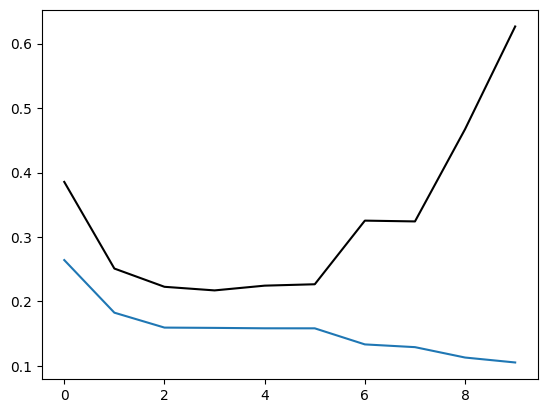
\includegraphics[width=400]{../assets/hw1_fig9.png}
\caption{Figure 9}
\end{figure}
Based on the plot, the polynomial degree that best fits the data appears to be around degree 2 or 3, as indicated by the lowest point of the test error curve (blue line). Before this point, underfitting is evident, where the model is too simple to capture the underlying data pattern. After this point, overfitting occurs, as the model complexity increases and the test error starts to rise, indicating that the model is fitting to the noise rather than the underlying relationship. The training error (black line) continues to decrease with increasing complexity, which is typical as more complex models can better fit the training data, but this does not generalize well to new data, as shown by the increasing test error.
\color{black}

\textbf{Regularization} \\[0pt]

Finally, we will explore the role of regularization. For this problem, we will use \(\ell_{2}\)
-regularization so that our regularized objective function is

$$
   J(\theta)=\frac{1}{2} \sum_{n=1}^{N}\left(h_{\theta}\left(\mathbf{x}_{n}\right)-y_{n}\right)^{2}+\frac{\lambda}{2}\left\|\theta_{[1: m]}\right\|^{2}
   $$

again optimizing for the parameters \(\theta\).

(h) Modify \texttt{loss\_and\_grad()} to incorporate \(\ell_{2}\) -regularization.

\color{teal}
See code appendix
\color{black}
\end{enumerate}


(i) Use your updated solver to find the coefficients that minimize the error for a tenth-degree polynomial \((m=10)\) given regularization factor \(\lambda=0,10^{-8}, 10^{-7}, \ldots, 10^{-1}, 10^{0}\). Now use these coefficients to calculate the loss (unregularized) on both the training data and test data as a function of \(\lambda\). Generate a plot depicting how the loss error varies with \(\lambda\) (for your x-axis, let \(x=[1,2, \ldots, 10]\) correspond to \(\lambda=\left[0,10^{-8}, 10^{-7}, \ldots, 10^{0}\right]\) so that \(\lambda\) is on a logistic scale, with regularization increasing as \(x\) increases). Which \(\lambda\) value appears to work best?

\begin{figure}[htbp]
\centering
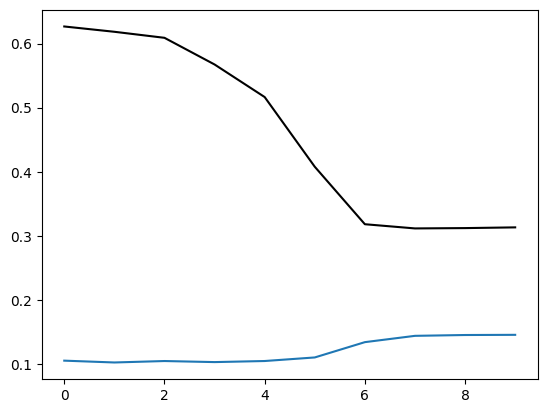
\includegraphics[width=400]{../assets/hw1_fig8.png}
\caption{Figure 8: Loss Variation with Lambda}
\end{figure}

\color{teal}
Out of all the values \(\lambda = 1\) appears to be the one that works best based off of the
graph
\color{black}





\textbf{Regression.py}
\begin{verbatim}
import numpy as np

class Regression(object):
    def __init__(self, m=1, reg_param=0):
        self.m = m
        self.reg = reg_param
        self.dim = [m+1, 1]
        self.w = np.zeros(self.dim)

    def gen_poly_features(self, X):
        num_samples, _ = X.shape
        degree = self.m
        poly_features = np.zeros((num_samples, degree+1))
        if degree == 1:
            poly_features[:, 0] = 1
            poly_features[:, 1] = X[:, 0]
        else:
            for i in range(num_samples):
                poly_features[i] = [X[i, 0]**deg for deg in range(degree + 1)]
        return poly_features
    
    def loss_and_grad(self, X, y):
        predictions = self.predict(X)
        poly_features = self.gen_poly_features(X)
        num_samples, _ = X.shape
        loss = np.mean((predictions - y) ** 2)
        gradient = 2 * poly_features.T.dot(predictions - y) / num_samples
        if self.m > 1:
            gradient += self.reg * np.r_[0, self.w[1:]]
        return loss, gradient

    def train_LR(self, X, y, eta=1e-3, batch_size=30, num_iters=1000) :
        loss_history = []
        N,d = X.shape
        for t in np.arange(num_iters):
                X_batch = None
                y_batch = None
                batch_indices = np.random.choice(N, batch_size, replace=False)
                for i in range(batch_size):
                    X_batch = X[batch_indices,:]
                    y_batch = y[batch_indices]
               
                loss = 0.0
                grad = np.zeros_like(self.w)
                self.w = self.w.flatten()
                loss, grad = self.loss_and_grad(X_batch, y_batch)
                self.w = self.w - eta*grad
                loss_history.append(loss)
        return loss_history, self.w

    def closed_form(self, X, y):
        poly_features = self.gen_poly_features(X)
        self.w = np.linalg.inv(poly_features.T @ poly_features + self.reg * np.eye(poly_features.shape[1])) @ poly_features.T @ y
        loss, _ = self.loss_and_grad(X, y)
        return loss, self.w
    
    def predict(self, X):
        poly_features = self.gen_poly_features(X)
        predictions = poly_features.dot(self.w).flatten()
        return predictions
\end{verbatim}





\textbf{Logistic.py}
\begin{verbatim}
import numpy as np

class LogisticRegression(object):
    def __init__(self, num_features=784, regularization_strength=0):
        self.regularization_strength = regularization_strength
        self.weights = np.zeros((num_features + 1, 1))

    def augment_features(self, X):
        num_samples = X.shape[0]
        return np.hstack([np.ones((num_samples, 1)), X])

    def compute_loss_and_gradient(self, X, y):
        augmented_X = self.augment_features(X)
        logits = np.dot(augmented_X, self.weights).flatten()
        probabilities = 1 / (1 + np.exp(-logits))
        binary_labels = (y + 1) / 2  # Convert from {-1, 1} to {0, 1}
        loss = -np.mean(binary_labels * np.log(probabilities) + (1 - binary_labels) * np.log(1 - probabilities))
        gradient = np.dot(augmented_X.T, (probabilities - binary_labels)) / num_samples
        if self.regularization_strength:
            gradient += self.regularization_strength * np.vstack([0, self.weights[1:]])
        return loss, gradient

    def train(self, X, y, learning_rate=1e-3, batch_size=1, num_iterations=1000):
        loss_history = []
        num_samples = X.shape[0]
        for _ in range(num_iterations):
            indices = np.random.choice(num_samples, batch_size, replace=False)
            X_batch = X[indices]
            y_batch = y[indices]
            loss, grad = self.compute_loss_and_gradient(X_batch, y_batch)
            self.weights -= learning_rate * grad
            loss_history.append(loss)
        return loss_history

    def predict(self, X):
        augmented_X = self.augment_features(X)
        logits = np.dot(augmented_X, self.weights)
        return np.where(logits > 0, 1, -1).flatten()
\end{verbatim}

\textbf{Notebook.ipynb}
\begin{verbatim}
# %%
import numpy as np
import matplotlib.pyplot as plt
import random
import csv
from utils import mnist_reader
from utils.data_load import load
import codes
# Load matplotlib images inline
%matplotlib inline
# These are important for reloading any code you write in external .py files.
# see http://stackoverflow.com/questions/1907993/autoreload-of-modules-in-ipython
%load_ext autoreload
%autoreload 2

# %% [markdown]
# # Problem 4: Binary Classification
# 
# Please follow our instructions in the same order to solve the binary classification problem.
# Please print out the entire results and codes when completed.

# %%
#X_train, y_train = mnist_reader.load_mnist('fashion-mnist/data/fashion', kind='train')
#X_test, y_test = mnist_reader.load_mnist('fashion-mnist/data/fashion', kind='t10k')

X_train = np.load('./data/binary_classification/X_train.npy')
y_train = np.load('./data/binary_classification/y_train.npy')
X_test = np.load('./data/binary_classification/X_test.npy')
y_test = np.load('./data/binary_classification/y_test.npy')

print('Train data shape: ', X_train.shape)
print('Train target shape: ', y_train.shape)
print('Test data shape: ',X_test.shape)
print('Test target shape: ',y_test.shape)

# %%
# PART (a): 
# To Visualize a point in the dataset
index = 11
X = np.array(X_train[index], dtype='uint8')
X = X.reshape((28, 28))
fig = plt.figure()
plt.imshow(X, cmap='gray')
plt.show()
if y_train[index] == 1:
    label = 'Dress'
else:
    label = 'Shirt'
print('label is', label)

# %% [markdown]
# ## Train Perceptron
# In the following cells, you will build Perceptron Algorithm.

# %%
# PART (b),(c): 
# Implement the perceptron Algorithm and compute the number of mis-classified point
N = X_train.shape[0] # Number of data point train
N_test = X_test.shape[0] # Number of data point test
d = X_train.shape[1] # Number of features
loss_hist = []
W = np.zeros((d+1,1))
X_train_h = np.hstack((np.ones((N,1)), X_train))
X_test_h = np.hstack((np.ones((N_test,1)), X_test))
# ================================================================ #
# YOUR CODE HERE:
# complete the following code to plot both the training and test accuracy in the same plot
# for m range from 1 to N
# ================================================================ #
test_loss_hist = []
W = W.flatten()
for i in range(N):
    x_i = X_train_h[i]
    y_i = y_train[i]
    y_pred = np.sign(np.dot(W, X_train_h[i]))
    if (y_pred != y_train[i]):
        W += y_train[i]* X_train_h[i]

        missclassified_train = 0
        missclassified_test = 0

        for j in range(N):
            train_pred = np.sign(np.dot(W, X_train_h[j]))
            if (train_pred != y_train[j]):
                missclassified_train += 1

        for k in range(N_test):
            test_pred = np.sign(np.dot(W, X_test_h[k]))
            if (test_pred != y_test[k]):
                missclassified_test += 1

        loss_hist.append(missclassified_train/N)
        test_loss_hist.append(missclassified_test/N_test)

    else:
        loss_hist.append(loss_hist[-1])
        test_loss_hist.append(test_loss_hist[-1])

# Print final losses
print(f'Final Loss Value (Train) = {loss_hist[-1]*100:.2f}%')
print(f'Final Loss Value (Test) = {test_loss_hist[-1]*100:.2f}%')
print(f'Norm of W = {np.linalg.norm(W)**2}')

# Plotting
plt.grid(True)
plt.plot(loss_hist, 'purple', label='Training Loss')
plt.plot(test_loss_hist, 'teal', label='Testing Loss')
plt.xlabel('Epochs')
plt.ylabel('Loss')
plt.title('Training and Testing Loss Over Epochs')
plt.legend()
plt.show()

# ================================================================ #
# END YOUR CODE HERE
# ================================================================ #

# %% [markdown]
# ## Train Logistic Regression
# In the following cells, you will build a logistic regression. You will implement its loss function, then subsequently train it with gradient descent.

# %%
from codes.Logistic import Logistic

# %%
## PART (f): 
X_train = np.load('./data/binary_classification/X_train.npy')
y_train = np.load('./data/binary_classification/y_train.npy')
X_test = np.load('./data/binary_classification/X_test.npy')
y_test = np.load('./data/binary_classification/y_test.npy')
## Complete loss_and_grad function in Logistic.py file and test your results.
N,d = X_train.shape
logistic = Logistic(d=d, reg_param=0)
loss, grad = logistic.loss_and_grad(X_train,y_train)
print('Loss function=',loss)
print(np.linalg.norm(grad,ord=2)**2)

# %%
# PART (h)
# Complete predict function in Logisitc.py file and compute the percentage of mis-classified points
y_pred = logistic.predict(X_test)
test_err = np.sum((y_test!=y_pred))*100/X_test.shape[0]
print(test_err,'%')

# %%
## PART (i): 
Batch = [1, 50 , 100, 200, 300]
test_err = np.zeros((len(Batch),1))
# ================================================================ #
# YOUR CODE HERE:
# Train the Logistic regression for different batch size. Average the test error over 10 times
# ================================================================ #

iters = 10
count = 0
for b in Batch:
    temp_err = 0
    for i in range(iters):
        logistic = Logistic(d = d)
        loss_hist, w = logistic.train_LR(X_train,y_train, eta=1e-5,batch_size=b, num_iters=6000/b)
        y_pred = logistic.predict(X_test)
        temp_err += np.sum((y_test!=y_pred))*100/X_test.shape[0]
            
    temp_err /= iters
    test_err[count] = temp_err
    count += 1

# ================================================================ #
# END YOUR CODE HERE
# ================================================================ #
fig = plt.figure()
plt.plot(Batch,test_err)
plt.xlabel('Batch_size')
plt.ylabel('Test_error')
plt.show()
fig.savefig('./plots/LR_Batch_test.pdf')

# %% [markdown]
# # Problem 5: Linear Regression
# Please follow our instructions in the same order to solve the linear regresssion problem.
# 
# Please print out the entire results and codes when completed.

# %%
def get_data():
    """
    Load the dataset from disk and perform preprocessing to prepare it for the linear regression problem.   
    """
    X_train, y_train = load('./data/regression/regression_train.csv')
    X_test, y_test = load('./data/regression/regression_test.csv')
    return X_train, y_train, X_test, y_test

X_train, y_train, X_test, y_test= get_data()  


print('Train data shape: ', X_train.shape)
print('Train target shape: ', y_train.shape)
print('Test data shape: ',X_test.shape)
print('Test target shape: ',y_test.shape)

# %%
## PART (a): 
## Plot the training and test data ##

plt.plot(X_train, y_train,'o', color='black')
plt.plot(X_test, y_test,'o', color='blue')
plt.xlabel('Train data')
plt.ylabel('Target')
plt.show()

# %% [markdown]
# ## Training Linear Regression
# In the following cells, you will build a linear regression. You will implement its loss function, then subsequently train it with gradient descent. You will choose the learning rate of gradient descent to optimize its classification performance. Finally, you will get the opimal solution using closed form expression.

# %%
from codes.Regression import Regression

# %%
## PART (c): 
## Complete loss_and_grad function in Regression.py file and test your results.
regression = Regression(m=1, reg_param=0)
loss, grad = regression.loss_and_grad(X_train,y_train)
print('Loss value',loss)
print('Gradient value',grad)
##

# %%
## PART (d) (Different Learning Rates):
from numpy.linalg import norm
lrs = [1e-1, 1e-2, 1e-3, 1e-4]
test_err = np.zeros((len(lrs),1))
# ================================================================ #
# YOUR CODE HERE:
# Train the Linear regression for different learning rates and average the test error over 10 times
# ================================================================ #
lrs = [1e-1, 1e-2, 1e-3, 1e-4]
test_err = np.zeros((len(lrs),1))  # This will store the average test error for each learning rate

# Loop over each learning rate
for index, eta in enumerate(lrs):
    errors = []  # To store the test errors for averaging

    # Repeat training and testing 10 times for each learning rate
    for _ in range(10):
        regression = Regression(m=1)  # Initialize the Regression object for linear regression
        # Train the model using the current learning rate
        regression.train_LR(X_train, y_train, eta=eta, batch_size=30, num_iters=1000)
        
        # Predict on test data
        y_pred = regression.predict(X_test)
        
        # Calculate the mean squared error for the test data
        error = np.mean((y_test - y_pred) ** 2)
        errors.append(error)

    # Average the test errors and store them
    test_err[index] = np.mean(errors)
# ================================================================ #
# END YOUR CODE HERE
# ================================================================ #
fig = plt.figure()
plt.plot(lrs,test_err)
plt.xlabel('Learning Rate')
plt.ylabel('Test_error')
plt.show()
fig.savefig('./plots/LR_Batch_test.pdf')

# %%
## PART (e): 
## Complete closed_form function in Regression.py file
loss_2, w_2 = regression.closed_form(X_train, y_train)
print('Optimal solution loss',loss_2)
print('Optimal solution gradient',w_2)

# %%
## PART (g): 
train_loss=np.zeros((10,1))
test_loss=np.zeros((10,1))
# ================================================================ #
# YOUR CODE HERE:
# complete the following code to plot both the training and test loss in the same plot
# for m range from 1 to 10
# ================================================================ #
for m in range(1,11):
    regression = Regression(m=m, reg_param=0)
    loss, w = regression.closed_form(X_train, y_train)
    train_loss[m-1] = loss
    y_pred = regression.predict(X_test)
    temp_loss = 0
    for i in range(X_test.shape[0]):
        temp_loss += (y_pred[i]-y_test[i])**2
    temp_loss /= X_test.shape[0]
    test_loss[m-1] = temp_loss

# ================================================================ #
# END YOUR CODE HERE
# ================================================================ #
plt.plot(train_loss)
plt.plot(test_loss, color='black')
plt.show()

# %%
#PART (i): 
train_loss=np.zeros((10,1))
test_loss=np.zeros((10,1))
# ================================================================ #
# YOUR CODE HERE:
# complete the following code to plot both the training and test loss in the same plot
# for m range from 1 to 10
# ================================================================ #
lambdas = [0, 1e-8, 1e-7, 1e-6, 1e-5, 1e-4, 1e-3, 1e-2, 1e-1, 1e0]
count = 0
for la in lambdas:
    regression = Regression(m=10, reg_param=la)
    loss, w = regression.closed_form(X_train, y_train)
    y_pred = regression.predict(X_test)
    temp_loss = 0
    for i in range(X_test.shape[0]):
        temp_loss += (y_pred[i]-y_test[i])**2
    temp_loss /= X_test.shape[0]
    train_loss[count] = loss
    test_loss[count] = temp_loss
    count += 1
# ================================================================ #
# END YOUR CODE HERE
# ================================================================ #

plt.plot(train_loss)
plt.plot(test_loss, color='black')
plt.show()



\end{verbatim}
\end{document}
